%%%%%%%%%%%%%%%%%%%%%%%%%%%%%%%%%%%%%%%%%
% TMDEI Dissertation
% LaTeX Template
% Version 0.1 (Dec/2015)
%
% Adapted to TMDEI/ISEP style (Dec/2015) by
%  Nuno Pereira (nap@isep.ipp.pt) and
%  Paulo Baltarejo (pbs@isep.ipp.pt)
%
% Based on MastersDoctoralThesis Version 1.2 by Vel (vel@latextemplates.com) and
% Johannes Böttcher, downloaded from (21/11/15):
% http://www.LaTeXTemplates.com
%
% This template is originally based on a template by:
% Steve Gunn (http://users.ecs.soton.ac.uk/srg/softwaretools/document/templates/)
% Sunil Patel (http://www.sunilpatel.co.uk/thesis-template/)
%
% Template license:
% CC BY-NC-SA 3.0 (http://creativecommons.org/licenses/by-nc-sa/3.0/)
%
%%%%%%%%%%%%%%%%%%%%%%%%%%%%%%%%%%%%%%%%%
%https://www.overleaf.com/project/5bfd7e508cfbf932785021c9
%----------------------------------------------------------------------------------------
%	PACKAGES AND OTHER DOCUMENT CONFIGURATIONS
%----------------------------------------------------------------------------------------

\documentclass[
11pt, % The default document font size, options: 10pt, 11pt, 12pt
%oneside, % Two side (alternating margins) for binding by default, uncomment to switch to one side (for drafting/reading purposes)
english, % english for English;
%portuguese,% for Portuguese; delete temporary files if you change language (e.g. 'make clean; make')
singlespacing, % Single line spacing, alternatives: onehalfspacing or doublespacing (for drafting/reading purposes)
%draft, % Uncomment to enable draft mode (no pictures, no links, overfull hboxes indicated)
%nolistspacing, % If the document is onehalfspacing or doublespacing, uncomment this to set spacing in lists to single
liststotoc, % Uncomment to add the list of figures/tables/etc to the table of contents (recommended)
%toctotoc, % Uncomment to add the main table of contents to the table of contents (not recommended)
parskip, % Add space between paragraphs (recommended)
%nohyperref, % Uncomment to not load the hyperref package (not recommended)
nohyperreflinkcolor, % hyperref links are not colored (comment to color links, for example to produce an electronic-only version)
headsepline, % Uncomment to get a line under the header
]{tmdei-style} % The class file specifying the document structure

\usepackage{comment} % To use comment in blocking

\usepackage[colorinlistoftodos]{todonotes}

\usepackage{tikz} % Required for creating graphics programmatically (can be removed if not used)
%\usetikzlibrary{arrows} % Required for fancy arrows in TiKZ graphics (can be removed if not used)

\usepackage{pgfplots} % Required for drawing high--quality function plots (can be removed if not used)
\pgfplotsset{compat=newest}

%
% Next you have examples of admissable citation styles; we recomend using the authoryear-comp citation style (which resembles Harvard); don't forget to only uncomment one
%

% authoryear-comp: recommended citation style (e.g. (Buendía, 1860), (Buendía 1910, Arcadio 1940))
%\usepackage[style=authoryear-comp,backend=biber]{biblatex} % Bibtex backend with the authoryear-comp citation style (authoryear citations, bibliography ordered alphabetically)

% numeric citation style (e.g. [1], [1-3])
\usepackage[style=numeric-comp,sorting=none,backend=biber]{biblatex} % Bibtex backend with the numeric-comp citation style (numeric citations, bibliography ordered by appearance)

% alphabetic citation style (e.g. [Buendía10], [Buendía10, Arcadio40])
%\usepackage[style=alphabetic,sorting=none,backend=biber]{biblatex} % Bibtex backend with the alphabetic citation style (alphabetic citations, bibliography ordered by appearance)

\addbibresource{references.bib} % The filename of the bibliography
\addbibresource{other_references.bib} % The filename of the bibliography

\makeglossaries % build the glossary

%----------------------------------------------------------------------------------------
%	THESIS INFORMATION
%----------------------------------------------------------------------------------------

\thesistitle{Comparative Analysis of Fault Tolerance in Elixir and Other Distributed Languages}% Your thesis title, this is used in the title, print it elsewhere with \ttitle

%\thesissubtitle{{[}Thesis Subtitle{]}} % Your thesis title, this is used in the title, print it elsewhere with \tsubtitle

\author{Nuno Ribeiro} % Your name, this is used in the title page, print it elsewhere with \authorname

\subjectarea{Software Engineering} % Specialisation area (Computer Systems, Information and Knowledge Systems, Graphics, Systems and Multimedia, Software Engineering), used in the title page, print it elsewhere with \areaname

\supervisor{Dr. Luís Nogueira} % Your advisors's name, this is used in the title page, print it elsewhere with \supname

%\cosupervisor{Dr. Jack \textsc{Smith}} % Your co-advisors's name, this is used in the title page, print it elsewhere with \cosupname (comment, if no co-supervisor)

% if committeepresident is defined, will add the thesis committee to the front page
%\committeepresident{Dr. Jonny Smith, Professor, DEI/ISEP} % Name of the president of the evaluation committee, print it elsewhere with \presidentname

%\committeemembers{Dr. Jaimie Smith, Professor, DEI/ISEP\\Dr. Jones Smith, Professor, DEI/ISEP\\Dr. Jagger Smith, Professor, DEI/ISEP} % Name of the evaluation committee members (up to four), print it elsewhere with \committee

\keywords{Keyword1, ..., Keyword6} % Please define up to 6 keywords that better describe your work, print it elsewhere with \keywordnames

\university{\href{https://www.isep.ipp.pt}{Instituto Superior de Engenharia do Porto}} % Your university's name and URL, this is used in the title page and abstract, print it elsewhere with \univname

\department{\href{http://department.university.com}{Department or School Name}} % Your department's name and URL, this is used in the title page and abstract, print it elsewhere with \deptname

\thesisdate{Porto, \today} % thesis date,  print it elsewhere with \tdate

\hypersetup{pdftitle=\ttitle} % Set the PDF's title to your title
\hypersetup{pdfauthor=\authorname} % Set the PDF's author to your name
\hypersetup{pdfkeywords=\keywordnames} % Set the PDF's keywords to your keywords

\begin{document}

%----------------------------------------------------------------------------------------
%	FRONT MATTER
%----------------------------------------------------------------------------------------

% Include the frontmatter of your thesis here
% we include the glossary here (frontmatter is included with \input, so this command is as if it was in main.tex)
%All acronyms must be written in this file.
\newacronym{IPC}{IPC}{Interprocess Communication}
\newacronym{URL}{URL}{Uniform Resource Locator}
\newacronym{RPC}{RPC}{Remote Procedure Call}
\newacronym{WWW}{WWW}{World Wide Web}
\newacronym{P2P}{P2P}{Peer to Peer}
\newacronym{IoT}{IoT}{Internet of Things}
\newacronym{ML}{ML}{Machine Learning}
\newacronym{AI}{AI}{Artificial Intelligence}
\newacronym{OTP}{OTP}{Open Telecom Platform}
\newacronym{CPU}{CPU}{Central Processing Unit}
\newacronym{CSP}{CSP}{Communicating Sequential Processes}
\newacronym{DSM}{DSM}{Distributed Shared Memory}
\newacronym{HTTP}{HTTP}{Hypertext Transfer Protocol}
\newacronym{gRPC}{gRPC}{Google Remote Procedure Call}
\newacronym{JVM}{JVM}{Java Virtual Machine}
\newacronym{WBS}{WBS}{Work Breakdown Structure}

 



\frontmatter % Use roman page numbering style (i, ii, iii, iv...) for the pre-content pages

\pagestyle{plain} % Default to the plain heading style until the thesis style is called for the body content

%----------------------------------------------------------------------------------------
%	TITLE PAGE
%----------------------------------------------------------------------------------------

\maketitlepage

%----------------------------------------------------------------------------------------
%	STATEMENT of INTEGRITY
%----------------------------------------------------------------------------------------
\integritystatement

%----------------------------------------------------------------------------------------
%	DEDICATION  (optional)
%----------------------------------------------------------------------------------------
%
%\dedicatory{For/Dedicated to/To my\ldots}
%\begin{dedicatory}
%The dedicatory is optional. Below is an example of a humorous dedication.

%\end{dedicatory}

%----------------------------------------------------------------------------------------
%	ABSTRACT PAGE
%----------------------------------------------------------------------------------------

\begin{abstract}

% here you put the abstract in the main language of the work.
Fault tolerance is a critical component of distributed systems, particularly in light of the exponential growth in internet usage and system scale in recent years. The resilience and fault tolerance capabilities of these systems are essential for maintaining reliability and minimizing downtime. Elixir, with its fault-tolerant features and its foundation in Erlang’s \textit{“let it crash”} philosophy, stands out as a robust tool for building such systems.

Nevertheless, other distributed and concurrent programming languages also offer solutions, often leveraging similar concepts in different environments. For instance, Akka, inspired by the \textit{“let it crash”} philosophy, provides a toolkit built for Scala. While both languages share conceptual foundations, Scala operates in a different environment with unique characteristics. Meanwhile, Go, a language gaining widespread popularity for its strong concurrency mechanisms, offers another compelling option for building concurrent and fault-tolerant systems.

Although all these languages can theoretically employ the Actor Model through libraries and toolkits, Elixir integrates these concepts natively, potentially providing distinct advantages. Conversely, Scala and Go include features that are not inherently available in Elixir’s Open Telecom Platform (OTP), such as replication on Akka, for example. Moreover, Go’s lack of native support for distributed systems raises questions about whether the advantages of using a widely adopted language can limiting on distributed computing compared with specific focus languages.

To investigate these assumptions and evaluate the comparative strengths and weaknesses of each language, benchmarking is necessary. Based on a review of existing literature, the most effective methodology, for this case, involves designing a generic application that simulates distributed operations sensitive to fault tolerance and resilience. This application will enable the creation of controlled test scenarios to yield measurable results, offering insights into the performance of each language in building fault-tolerant systems.

Future work will focus on implementing the benchmarking strategies, collecting performance, fault tolerance, and resilience metrics, as well as static code metrics. These efforts will be supported by detailed project planning to ensure the successful execution and meaningful outcomes of the project.

\end{abstract}

\begin{abstractotherlanguage}
% here you put the abstract in the "other language": English,m if the work is written in Portuguese; Portuguese, if the work is written in English.

% Para alterar a língua basta ir às configurações do documento no ficheiro \file{main.tex} e alterar para a língua desejada ('english' ou 'portuguese')\footnote{Alterar a língua requer apagar alguns ficheiros temporários; O target \keyword{clean} do \keyword{Makefile} incluído pode ser utilizado para este propósito.}. Isto fará com que os cabeçalhos incluídos no template sejam traduzidos para a respetiva língua.

A tolerância a falhas é um componente fundamental dos sistemas distribuídos, especialmente tendo em conta o grande crescimento da utilização da Internet e a crescente necessidade de sistemas mais robustos nos últimos anos. As capacidades de resiliência e tolerância a falhas destes sistemas são essenciais para garantir a fiabilidade e minimizar o tempo de inatividade devido a falhas. Elixir, com as suas características de tolerância a falhas e tendo a sua base na filosofia \textit{“let it crash”} de Erlang, destaca-se como uma ferramenta poderosa para a construção desses sistemas. Elixir herda todas as capacidades do Erlang, assim como da sua \textit{virtual machine}, sendo projetado para garantir alta disponibilidade nos diversos sistemas em que é utilizado, como, por exemplo, em bancos e telecomunicações.

Contudo, outras linguagens de programação distribuídas e concorrentes também oferecem soluções, muitas vezes aproveitando conceitos semelhantes em ambientes distintos, ou até mesmo inspirando-se na solução oferecida por Elixir, adaptando-a aos seus próprios conceitos, ou utilizando abordagens diferentes mas com objetivos semelhantes. Por exemplo, o Akka, inspirado pela filosofia \textit{“let it crash”}, fornece um conjunto de ferramentas criado para Scala, permitindo imitar o comportamento visto em Elixir com o uso de padrões \textit{supervisor}. Embora ambas as linguagens compartilhem a mesma filosofia, o Scala opera num ambiente diferente, com características únicas, funcionando sobre a \textit{Java Virtual Machine} (JVM). Por outro lado, Go, uma linguagem que tem ganho popularidade devido aos seus mecanismos de concorrência robustos e ao seu uso em vários projetos de grande escala, adota uma abordagem diferente e oposta quanto ao controlo de erros, sendo mais explícita e rejeitando a ideia de que os erros devem ser encarados como inevitáveis, sem a necessidade de um controlo tão refinado dentro dos componentes.

Embora todas estas linguagens possam teoricamente empregar o \textit{Actor Model} através de bibliotecas e kits de ferramentas, como o Akka em Scala e o Proto-Actor em Go, Elixir integra esses conceitos de forma nativa, o que pode oferecer vantagens distintas. Por outro lado, Scala e Go incluem funcionalidades que não estão presentes de forma nativa na \textit{Open Telecom Platform} (OTP) do Elixir. Além disso, a falta de suporte nativo de Go para sistemas distribuídos levanta questões sobre a conveniência de utilizar uma linguagem amplamente adotada, mas com limitações na computação distribuída, quando comparada com linguagens mais específicas para esse fim. Assim, o objetivo é perceber se, para a criação de um sistema tolerante a falhas, a utilização de uma linguagem nativa como o Elixir compensa em comparação com a utilização de uma linguagem mais genérica, mas com maior popularidade.

Para investigar estes pressupostos e avaliar as vantagens e desvantagens de cada linguagem, será necessário realizar uma avaliação comparativa através de \textit{benchmarking}. Com base numa revisão da literatura existente, a metodologia mais eficaz para este caso envolve a criação de uma aplicação genérica que simule operações distribuídas sensíveis à tolerância a falhas e resiliência. Esta abordagem, combinando diferentes métodos utilizados na literatura, permitirá a criação de cenários de teste controlados em sistemas que tentam imitar processos reais, gerando resultados mensuráveis.

O trabalho futuro concentrar-se-á na implementação de um \textit{benchmarking} detalhado, na análise e recolha de métricas, bem como na apresentação das conclusões. A abordagem proposta envolve o desenvolvimento de uma aplicação de \textit{chat} que suporte funcionalidades básicas, sendo implementada nas três linguagens selecionadas. No caso da linguagem Go, serão realizadas duas implementações: uma utilizando o \textit{Actor Model} através do \textit{toolkit} Proto-Actor e outra adotando abordagens nativas para distribuição e mecanismos de tolerância a falhas próprios da linguagem e de bibliotecas externas.

A execução desta análise permitirá a obtenção de métricas relacionadas ao desempenho, tolerância a falhas e resiliência, complementadas por uma análise estática do código. Estes esforços serão conduzidos com o apoio de um planeamento detalhado, no qual todas as fases do projeto estão descritas e os entregáveis devidamente definidos, garantindo assim uma execução planeada e controlada.

\end{abstractotherlanguage}

%----------------------------------------------------------------------------------------
%	ACKNOWLEDGEMENTS (optional)
%----------------------------------------------------------------------------------------

% \begin{acknowledgements}

% The optional Acknowledgment goes here\ldots Below is an example of a humorous acknowledgment.

%\end{acknowledgements}

%----------------------------------------------------------------------------------------
%	LIST OF CONTENTS/FIGURES/TABLES PAGES
%----------------------------------------------------------------------------------------

\tableofcontents % Prints the main table of contents

\listoffigures % Prints the list of figures

\listoftables % Prints the list of tables

\begin{comment}
\iflanguage{portuguese}{
\renewcommand{\listalgorithmname}{Lista de Algor\'itmos}
}
\listofalgorithms % Prints the list of algorithms
\addchaptertocentry{\listalgorithmname}



\renewcommand{\lstlistlistingname}{List of Source Code}
\iflanguage{portuguese}{
\renewcommand{\lstlistlistingname}{Lista de C\'odigo}
}
\lstlistoflistings % Prints the list of listings (programming language source code)
\addchaptertocentry{\lstlistlistingname}
\end{comment}


%----------------------------------------------------------------------------------------
%	ABBREVIATIONS
%----------------------------------------------------------------------------------------
%\begin{abbreviations}{ll} % Include a list of abbreviations (a table of two columns)
%%\textbf{LAH} & \textbf{L}ist \textbf{A}bbreviations \textbf{H}ere\\
%%\textbf{WSF} & \textbf{W}hat (it) \textbf{S}tands \textbf{F}or\\
%\end{abbreviations}

%----------------------------------------------------------------------------------------
%	SYMBOLS
%----------------------------------------------------------------------------------------

%\begin{symbols}{lll} % Include a list of Symbols (a three column table)

%$a$ & distance & \si{\meter} \\
%$P$ & power & \si{\watt} (\si{\joule\per\second}) \\
%Symbol & Name & Unit \\

%\addlinespace % Gap to separate the Roman symbols from the Greek

%$\omega$ & angular frequency & \si{\radian} \\

%\end{symbols}



%----------------------------------------------------------------------------------------
%	ACRONYMS
%----------------------------------------------------------------------------------------

\newcommand{\listacronymname}{List of Acronyms}
\iflanguage{portuguese}{
\renewcommand{\listacronymname}{Lista de Acr\'onimos}
}

%Use GLS
\glsresetall
\printglossary[title=\listacronymname,type=\acronymtype,style=long]

%----------------------------------------------------------------------------------------
%	DONE
%----------------------------------------------------------------------------------------

\mainmatter % Begin numeric (1,2,3...) page numbering
\pagestyle{thesis} % Return the page headers back to the "thesis" style


%----------------------------------------------------------------------------------------
%	MAIN BODY
%----------------------------------------------------------------------------------------

% Include the chapters of the thesis as separate folder for each chapter
% Uncomment the lines as you write the chapters

% Chapter 1
% 
\chapter{Introduction} % Main chapter title
\label{chap:Chapter1} % For referencing the chapter elsewhere, use Chapter~\ref{Chapter1}


%-------------------------------------------------------------------------------
%---------
%
\section{Context} 

\section{Problem}

\section{Objectives}

\section{Ethics}

\section{Document structure} 
% Chapter 2

\chapter{Background} % Main chapter title

\label{chap:Chapter2} % For referencing the chapter elsewhere, use \ref{chap:Chapter2} 

%----------------------------------------------------------------------------------------

\section{Distributed Systems}

In the early days of computing, computers were large and expensive, operating as standalone machines without the ability to communicate with each other. As technology advanced, smaller and more affordable computers, such as smartphones and other devices, were developed, along with high-speed networking that allowed connectivity across a network \cite{Tanenbaum2023}. These innovations made it possible to create systems distributed across nodes where tasks could be processed collectively to achieve a common goal \cite{Sharma2016}. Nodes in a distributed system may refer to physical devices or software processes\cite{Vitillo2021}.

To the end-user, distributed systems appear as a single, large virtual system, making the underlying logic transparent \cite{Naik2021}. These systems achieve a shared objective by transmitting messages through various nodes and dividing computational tasks among them, increasing resilience and isolating business logic \cite{Lamport1978, Sari2015, Vitillo2021}. Distributed systems can present heterogeneity, such as differing clocks, memory, programming languages, operating systems, or geographical locations, all of which must be abstracted from the end-user \cite{Sari2015, Tanenbaum2023}.

While decentralized and distributed systems share characteristics, they differ in node organization and governance. Distributed systems spread nodes across computers to improve reliability and scalability, distributing logic without centralization \cite{Tanenbaum2023}. For example, email systems scale with user demand without needing consensus. In contrast, decentralized systems, like blockchain, involve independent nodes with shared authority, requiring consensus for key operations to ensure trust \cite{aws-decentralization,Tanenbaum2023}. This document will focus on distributed systems.

Distributed systems are widely used across various fields, including banking and healthcare, and are the focus of ongoing research as they expand into emerging areas like cloud and edge computing \cite{Brendan2018, Coulouris2012, Lindsay2021}. Their evolution is driven by the numerous advantages they offer, such as scalability, reliability, and transparency when well-structured. However, these benefits also introduce new challenges, increasing the complexity of debugging and testing, for example \cite{Brendan2018}. The following subsections will provide a detailed exploration of these aspects.

\subsection{Characteristics}

On a distributed system, when being well-structured, it is possible to find, among others, the following most popular characteristic:

\subsubsection{Transparency}

Due to their transparency, distributed systems allow end-users interact with them without them realizing how complex they are \cite{Tanenbaum2023, Ledmi2018}. This trait is called transparency, and it can manifest in a variety of ways. These consist of:

\begin{enumerate}
    \item \textbf{Access transparency}: This enables resources to be accessed seamlessly across different nodes, whether local or remote, while hiding differences such as operating systems, programming languages, or other implementation details \cite{Tanenbaum2023, Coulouris2012}.
    
    \item \textbf{Location transparency}: This hides the physical location of resources or nodes, allowing users to access them without needing to know where they are located. For example, a \gls{URL} provides location transparency by enabling users to access a resource abstracting the physical location \cite{Tanenbaum2023, Banatre1991}.
    
    \item \textbf{Relocation transparency}: This ensures that if a resource or node is moved to a new physical location, the change is invisible to users. For instance, if a website is relocated, its \gls{URL} remains the same \cite{Tanenbaum2016}.
    
    \item \textbf{Mobility transparency}: This allows both clients and resources to move without disrupting ongoing operations for users or applications. An example of mobility transparency is a mobile phone call, where communication remains unaffected even if the involved are moving \cite{Coulouris2012, Tanenbaum2016}.
    
    \item \textbf{Replication transparency}: This hides the replication of resources or nodes, which may occur to improve reliability and availability. For instance, a distributed file system may replicate data to ensure availability even if one copy becomes inaccessible \cite{Tanenbaum2023}.
    
    \item \textbf{Concurrency transparency}: This allows multiple processes to operate concurrently without conflict, even if they share the same physical resources \cite{Coulouris2012}.
    
    \item \textbf{Failure transparency}: This enables the system to continue functioning despite certain failures, making these issues invisible to users while ensuring that tasks are completed as intended \cite{Coulouris2012}.
\end{enumerate}

\subsubsection{Reliability and availability}

A distributed system should have reliability and availability aspects. Reliability refers to its ability to continuously perform its intended requirements without interruption, operating exactly as designed, even in the presence of certain internal failures \cite{Ahmed2013}. A highly reliable system maintains consistent, uninterrupted service over an extended period, minimizing disruptions for users \cite{Tanenbaum2023}. On other hand, availability measures the probability that the system is operational and ready to respond correctly at any given moment, often expressed as a percentage of system up-time \cite{Tanenbaum2023, atlassian-availability}. 

\subsubsection{Scalability}

Designing and building a distributed system is complex, but also enables the creation of highly scalable systems, capable of expanding to meet increasing demands \cite{Tanenbaum2023, Vitillo2021, Valkov2018}. This characteristic is particularly evident as cloud-based systems become more popular, allowing users to interact with applications over the internet rather than relying on local desktop computing power \cite{Lindsay2021}. Cloud services must support a large volume of simultaneous connections and interactions, making scalability a crucial factor \cite{Tanenbaum2023}.

\begin{quote}
	\textit{"A system is described as scalable if it will remain effective when there is a significant increase in the number of resources and the number of users."} \cite{Coulouris2012}
\end{quote}

Scalability can be addressed across three dimensions: size scalability allows for additional users and resources without loss in performance, geographical scalability maintains performance despite physical distance between nodes, and administrative scalability manages increasing complexity as nodes take on distinct management roles \cite{Tanenbaum2023}.

%%%%%% BLOCK COMMENT %%%%%%
\begin{comment}
In distributed systems, scalability can be approached in three distinct dimensions \cite{Tanenbaum2023}:

\begin{enumerate}
	\item \textbf{Size scalability}: This allows the system to accommodate additional resources and users without a decrease in performance or reliability, ensuring that the system continues to deliver the expected results.
	      	      	      	      
	\item \textbf{Geographical scalability}: This dimension addresses the ability to maintain system performance despite the physical distance between users and resources. Geographical scalability mitigates latency and network constraints that may arise due to long distance communication.
	      	      	      	      
	\item \textbf{Administrative scalability}: This type of scalability enables the system to handle increasing administrative complexity, such as when separate nodes have different management responsibilities. For example, one set of nodes might handle financial transactions only adding the fact of allowing write-only operations to a specific range os users. As these constraints and requirements grow, the system must adapt to maintain efficient operation.
\end{enumerate}
\end{comment}

\subsubsection{Fault tolerance}

Fault tolerance is a critical characteristic of distributed systems, closely linked to reliability, availability, and scalability. For a system to maintain these properties, it must be able to mask failures and continue operating despite the presence of errors \cite{Strigini2012}. Fault tolerance is especially vital in distributed environments where system failures can lead to significant disruptions and economic losses across sectors such as finance, telecommunications, and transportation \cite{Sari2015}.

The primary goal of a fault-tolerant system is to enable continuous operation by employing specific strategies and design patterns to mask the possible errors \cite{Kleppmann2017}. Due to the importance of this topic to the dissertation, fault tolerance it will be detailed on the next chapter.

\subsection{Communication}

In distributed systems, communication between nodes is crucial for coordination and data exchange. When nodes are separated by a network, communication occurs over that network, whereas nodes on the same machine uses \gls{IPC} (Inter-Process Communication) \cite{Vitillo2021}. Network-based communication can introduce delays or be unreliable, making asynchronous communication advantageous in many situations \cite{Yuan2020}. However, some scenarios require synchronous communication for immediate feedback.

\subsubsection{Synchronous and asynchronous communication}

In synchronous communication, the sender waits for a response before continuing, making it a blocking operation \cite{Tanenbaum2023, Coulouris2012}. This method is helpful when the sender requires confirmation or feedback to proceed.

Asynchronous communication, by contrast, enables the sender to continue processing without waiting for a response, supporting a non-blocking flow \cite{Tanenbaum2023, Glabbeek2008}. This approach is well-suited to systems with high heterogeneity or where decoupling is essential, often implemented with message queues that provide transparency between sender and receiver \cite{Tanenbaum2023}.

\subsubsection{Communication models}

Within synchronous and asynchronous types, several communication models exist:

\textit{\gls{RPC}}

\gls{RPC} supports location transparency, allowing the sender to make a request to a remote node as if the call were local, within the same process or environment \cite{Kleppmann2017, Coulouris2012}. This is achieved through a mechanism known as a stub, which handles request and response processes on both client and server sides, ensuring data parsing and call transparency over the network \cite{Tanenbaum2023}.

\textit{Message passing}

In message passing, data is encapsulated into a message and sent to a queue on the receiver’s side. This model typically follows an asynchronous approach, where the sender does not expect an immediate reply \cite{Kleppmann2017, Coulouris2012}. However, message passing can also be synchronous if the sender requires an acknowledgment of receipt \cite{Coulouris2012}. Communication via message passing can be managed by a broker, such as RabbitMQ,\footnote{«Official website of RabbitMQ». \url{https://www.rabbitmq.com/} (accessed 02 November 2024)}, for example, or implemented natively, as seen in Erlang’s messaging passing system \cite{Nystrom2009, Tanenbaum2023}.

\subsection{Challenges}

Distributed systems encounter numerous challenges, including scalability \cite{Ahmed2013}, managing software, network, and disk failures \cite{Naik2021, aws-challenges-dist-sys}, heterogeneity \cite{Coulouris2012}, coordination among nodes \cite{Vitillo2021}, and difficulties on debugging and testing \cite{Beschastnikh2020, aws-challenges-dist-sys}. For the scope of this dissertation only the CAP theorem will be discussed.

\subsubsection{CAP theorem}

The CAP theorem says that in a system where nodes are networked and share data, it is impossible to simultaneously achieve all three properties of Consistency, Availability, and Partition Tolerance \cite{Tanenbaum2023, Vitillo2021}. This theorem underlines a critical trade-off in distributed systems: only two of these properties can be fully ensured at any given time \cite{ibm-cap-theorem, Gilbert2012}. A description of the properties can be given by:

\begin{itemize}
	\item \textbf{Consistency:} Ensures that all nodes in the system reflect the same data at any time, so each read returns the latest write.
	\item \textbf{Availability:} Guarantees that every request receives a response, whether successful or not, even if some nodes are offline.
	\item \textbf{Partition tolerance:} Allows the system to continue operating despite network partitions, where nodes may temporarily lose the ability to communicate.
\end{itemize}

According to the CAP theorem, when a network partition occurs, a distributed system must prioritize either consistency or availability, as achieving all three properties is not feasible in practice \cite{Tanenbaum2023, ibm-cap-theorem, Vitillo2021}. This concept is directly relevant to this dissertation, as fault tolerance strategies discussed later will account for these trade-offs to optimize specific properties.

\subsection{Evolution of distributed systems}

Distributed systems have been a significant area of research in computer science. The journey began with early client-server models in mainframe computing, which allowed virtualization to increase efficiency, which is an popular approach still in use today \cite{Lindsay2021}. This was followed by the development of cluster computing, offering affordable ways to boost computing power without relying on costly mainframes \cite{Lindsay2021, Gill2024}. During this phase, the Internet and the \gls{WWW} were created, marking an important point in history \cite{Lindsay2021}.

Subsequently, \gls{P2P} systems emerged, decentralizing computing through cooperative and distributed processes. With the rise of cloud computing, mobile computing, and the \gls{IoT} reached new levels of scalability, flexibility, and accessibility \cite{Gill2024}. Another design that emerged is micro-services architecture, which shares many properties with distributed systems and is widely used on the industry \cite{Adbelfattah2023}. Today, cutting-edge advancements focus on the following paradigms \cite{Gill2024}:

\begin{itemize}
	\item \textbf{Edge Computing:} Extends computing resources closer to data sources and end users, reducing latency and improving performance in real-time applications. This approach is critical for \gls{IoT} and applications where immediacy is essential \cite{Cao2020, Lindsay2021, Gill2024}.
	\item \textbf{Fog Computing:} Provides a layer of computing power between the cloud and edge devices, enhancing processing capabilities closer to the data source \cite{Cao2020, Lindsay2021, Gill2024}.
	\item \textbf{Dew Computing:} Complements cloud, edge, and fog computing by enabling local devices to perform data processing even when disconnected from centralized resources, enhancing resilience and accessibility for remote or offline scenarios \cite{Gusev2021, Gill2024}.
	\item \textbf{Serverless Computing:} Enables developers to execute code without managing underlying servers, automatically scaling resources based on demand. This model reduces operational overhead and allows efficient, event-driven architectures \cite{Yongkang2023, Gill2024}.
\end{itemize}

    
%%%%%%%%%%%%%%%%%%%%%%%%%%% FAULT TOLERANCE %%%%%%%%%%%%%%%%%%%%%%%%%%%

\section{Fault Tolerance}

With the extensive use of software systems across various domains, such as banking, transportation, and more, the demand for reliable and available systems is increasingly essential. However, errors in software are inevitable, making fault tolerance a critical attribute for systems to continue functioning correctly even in the presence of failures \cite{Sari2015}. Fault tolerance can address a range of issues, including networking, hardware, software, and other dimensions, with various strategies designed to manage these different fault types \cite{Sharma2016,Noor2019}.

\subsection{Fault Tolerance Taxonomy}

It is important to classify and understand the types of faults and failures that can arise. This section presents a taxonomy of fault tolerance concepts, drawing on the framework proposed by Isukapalli et al.\cite{Isukapalli2024}. A fault is defined as an underlying defect within a system component that may lead to an error, which is a deviation from the intended internal state. If this error remains unresolved, it may escalate into a system failure, potentially impacting system functionality either partially or completely \cite{Isukapalli2024,Reghenzani2023}. 

Table \ref{tab:fault_types} provides a classification of faults that commonly arise in fault tolerant systems. Each type requires different strategies for detection and mitigation, depending on the nature and persistence of the fault \cite{Isukapalli2024,Tanenbaum2023}.

Failures, on the other hand, are the external manifestations of these internal faults, as outlined in Table \ref{tab:failure_types}. These include crash failures, where the system halts entirely, to arbitrary failures, where responses are erratic and potentially misleading \cite{Tanenbaum2023,Haider2011}.

\begin{table}[h!]
    \centering
    \begin{tabular}{|l|p{10.8cm}|}
        \hline
        \textbf{Fault Type} & \textbf{Description} \\ \hline
        Transient Faults & Temporary faults that occur one time and retrying or restarting the operation the problem it disappear \cite{Reghenzani2023,Tanenbaum2023}. \\ \hline
        Intermittent Faults & Faults that appear sporadically, similar to transient faults, but with a higher persistence often due to hardware or environmental factors (e.g., temperature fluctuations affecting a hard disk) \cite{Reghenzani2023,Isukapalli2024}. \\ \hline
        Permanent Faults & Persistent faults caused by a complete failure of a system component. These faults remain until the root cause is identified and corrected, making them relatively straightforward to fix \cite{Reghenzani2023}. \\ \hline
    \end{tabular}
    \caption{Types of Faults and Their Descriptions}
    \label{tab:fault_types}
\end{table}

\begin{table}[h!]
	\centering
	\begin{tabular}{|l|p{11cm}|}
		\hline
		\textbf{Type of Failure} & \textbf{Description} \\ \hline
		Crash Failure            & The system halts and stops all operations entirely. Although it was functioning correctly before the halt, it does not resume operations or provide responses after the failure. \cite{Tanenbaum2023} \\ \hline
		Omission Failure         & The system fails to send or receive necessary messages, impacting communication and task coordination. \cite{Haider2011} \\ \hline
		Timing Failure           & The system’s response occurs outside a specified time interval, either too early or too late, causing issues in time-sensitive operations. \cite{Isukapalli2024} \\ \hline
		Response Failure         & The system provides incorrect outputs or deviates from expected state transitions, potentially leading to erroneous results. \cite{Tanenbaum2023} \\ \hline
		Arbitrary Failure        & The system produces random or unpredictable responses at arbitrary times, potentially with incorrect or nonsensical data. This type of failure is challenging to diagnose and manage. \cite{Tanenbaum2023} \\ \hline
	\end{tabular}
	\caption{Brief Description of Failure Types}
	\label{tab:failure_types}
\end{table}


\subsection{Strategies}

Various strategies and mechanisms can be applied to a system to achieve fault tolerance, and these must be chosen to suit the specific system type. This dissertation will primarily focus on software fault tolerance strategies, and focused on those suitable for the distributed languages bellow presented. Therefore, next it will be shown some strategies that it will serve as a theoretical basis for some of techniques that it will be used.

\subsubsection{Retry}

The retry strategy is a popular and straightforward technique that involves repeating an operation that initially failed, under the assumption that it might succeed upon retry \cite{Ledmi2018,Noor2019}. This strategy may include configurations like a back-off delay between attempts, but its fundamental principle remains the same.

\subsubsection{Replication}

Replication is a technique aimed at masking errors by creating redundant task clones. In this approach, multiple replicas of a job run simultaneously, acting as a group that performs the same operations. This redundancy allows the system to provide a response even in the event of a host, network, or other types of errors. Replication strategies can vary in communication modes, which may be synchronous or asynchronous. In some cases, a consensus algorithm is needed to reach a final decision among the replicas \cite{Isukapalli2024,Tanenbaum2023,Ledmi2018}.

\subsubsection{Check-pointing and Message Logging}

The check-pointing strategy periodically saves the state of a process so that, in the event of a failure, the process can restart from the last saved state, or "checkpoint," rather than start all over. This approach reduces the need to repeat the entire operation \cite{Isukapalli2024,Coulouris2012}.

Message logging is a lighter-weight approach with a similar goal. Instead of saving entire checkpoints, it records all the necessary messages that lead the process to a specific state. In case of a failure, the messages are replayed in the same order, guiding the system back to the desired state \cite{Ledmi2018}.

\subsection{Evolution and the State-of-the-Art}

\todo[]{ajustar isto}

Fault tolerance has significantly evolved, with substantial advancements in both software and hardware techniques. As studied by Arshad A. et al. \cite{Hussein2021}, recent developments focus on leveraging novel technologies to enhance system resilience. Furthermore, with \gls{AI} and \gls{ML} has introduced predictive fault tolerance techniques that aim to anticipate and mitigate faults before they lead to system failures.

Current strategies can be categorized into three types:

\begin{itemize}
	
	\item \textbf{Reactive Strategies}: These methods aim to reduce the impact of faults after they occur. For instance, techniques like task migration on processor level \cite{Fochi2021} and checkpoint/restart mechanisms \cite{Hussain2021} allow systems to recover by either transferring tasks or restarting operations from saved states.
	      
	\item \textbf{Proactive Strategies}: Proactive methods focus on preventing faults by monitoring system conditions and taking preemptive actions. For example, Fayyaz et al. proposed a distributed satellite architecture that integrates fault-tolerant performance measurements to manage processor faults effectively \cite{Fayyaz2018}.
	      
	\item \textbf{Predictive Strategies}: With advancements in \gls{AI} and \gls{ML}, predictive fault tolerance has emerged as a cutting-edge approach, wherein algorithms forecast potential failures and initiate corrective measures. For instance, Ghosh et al. utilized a fault management subsystem within a transactive energy application to improve system resilience by analyzing interaction patterns \cite{Ghosh2021}.
	      
\end{itemize}

Several innovative techniques have been proposed to address specific challenges in fault tolerance. Examples include the use of erasure coding in distributed file systems to balance storage costs and redundancy \cite{Arafa2021}, adaptive learning for fault detection in multi-agent systems \cite{Khalili2021}, and circuit breaker patterns for fault recovery in stream processing architectures \cite{Knasmueller2021}. 

%%%%%%%%%%%%%%%%%%%%%%%%%%% Distributed Programming Languages %%%%%%%%%%%%%%%%%%%%%%%%%%%


\section{Distributed and Concurrency Programming}

Distributed and concurrent programming languages play an important role in building resilient, scalable, and fault-tolerant systems \cite{Armstrong2013}. In distributed systems, where components operate across multiple nodes, and in concurrent systems, where tasks can execute in parallel on the same machine's \gls{CPU}, programming languages must provide mechanisms to manage faults effectively. These mechanisms should isolate faults to prevent cascading failures, at the same time ensuring overall system reliability and availability \cite{Nystrom2009}, or should have forms to equip the language with capacities to handle this type of systems.

The evolution of distributed programming languages has been driven by the need to address the complexities of developing distributed systems, which include issues such as concurrency, parallelism, fault tolerance, and secure communication. This has driven the evolution of new paradigms, languages, frameworks, and libraries aimed at reducing development complexity in distributed and concurrent systems \cite{Valkov2018}.

\subsection{Models and Paradigms}

The field of distributed programming has been shaped by research and development in concurrency and parallelism, and some models and paradigms have been developed to address this challenge, where some ideas had some focus restricted to the research others have been addressed to the industry. In the following it will be described the models and paradigms that bring interest to this dissertation:
\subsubsection{Actor Model}

The Actor Model, a conceptual framework for concurrent and distributed computing, was introduced by Carl Hewitt in 1973 \cite{Hewitt1973}. It defines a communication paradigm where an actor, the fundamental unit of computation, interacts with other actors exclusively through asynchronous message passing, with messages serving as the basic unit of communication \cite{Trinder2017}. Each actor is equipped with its own mailbox, which receives messages and processes them sequentially \cite{Koster2016}.

A core principle of the Actor Model is isolation, maintaining their own internal state that is inaccessible and immutable by others \cite{Koster2016}. This eliminates the need for shared memory, reducing complexity and potential data races. Another key feature is location communication, which allows actors to communicate seamlessly regardless of their physical location, whether on the same machine or across a distributed network. This transparency is achieved because all interactions are inherently message-based \cite{Trinder2017}.

The Actor Model also introduces the concept of supervision, where actors can monitor the behavior of other actors and take corrective actions in the event of a failure. This supervisory mechanism significantly enhances fault tolerance, enabling systems to recover gracefully from errors without compromising overall reliability \cite{Trinder2017}.

The Actor Model has been instrumental in shaping distributed system design and has been natively implemented in programming languages such as Erlang, Clojure and Elixir \cite{Randtoul2022}. Additionally, the model has been extended to other languages through frameworks and libraries. For instance, Akka brings actor-based concurrency to Scala, C\texttt{\#} and F\texttt{\#} while Kilim offers similar functionality for Java \cite{Trinder2017}. Comparable patterns can also be adopted in other languages like Go, Rust, and Ruby using libraries or custom abstractions.


\subsubsection{\gls{CSP}}

The field of distributed computing emphasizes mathematical rigor in algorithm analysis, with one of the most influential models being Communicating Sequential Processes (\gls{CSP}), introduced by C.A.R. Hoare in 1978 \cite{Hoare1983}.

\todo[inline]{refs}

\gls{CSP} offers an abstract and formal framework for modeling interactions between concurrent processes through channels, which serve as the communication medium between them \cite{Paduraru2018}. Processes operate independently, but they are coupled via these channels, and communication is typically synchronous, requiring the sender and receiver to synchronize for message transfer. While similar in some respects to the Actor Model, \gls{CSP} distinguishes itself through its emphasis on direct coupling via channels and strict synchronization \cite{}.

The \gls{CSP} model has had a profound influence on programming languages and frameworks. For example, Go integrates \gls{CSP} concepts in its implementation of goroutines and channels, enabling structured concurrency and communication \cite{go-docs, Valkov2018}. Additionally, the language Occam offers a more direct and faithful realization of \gls{CSP} principles, making it a pioneering choice \cite{Brolos2021}.

\subsubsection{Microservices Architectures}

Despite extensive research in distributed programming languages, many have not achieved widespread adoption in industry \cite{}. As a result, a new approach for designing distributed systems has emerged: microservices architectures. This paradigm shifts the focus to a higher level of abstraction, making the architecture language-agnostic by decomposing a system into a collection of loosely coupled services, each responsible for a specific function. These services interact using lightweight protocols such as HTTP/REST, gRPC, or message queues, promoting separation of concerns, modularity, and flexibility \cite{Fowler2014}.

This design approach has enabled general-purpose programming languages to compete with, and sometimes complement, native distributed programming paradigms. By combining robust frameworks or libraries with microservices principles, these languages can facilitate the development of distributed and fault-tolerant systems, bridging the gap between traditional distributed models and modern software architecture practices. In some cases, microservices architectures even incorporate features from native paradigms, merging their strengths to create scalable, resilient systems.

\subsubsection{Comparison of Models and Paradigms}


\subsection{Distributed and Concurrent Programming Languages}


\subsubsection{Analyses and Justification}

\begin{comment}


The Shared-Nothing Architecture (SNA) is a design principle that ensures each component in a system operates independently, with no shared memory or storage. Communication is achieved through explicit message passing or synchronization mechanisms. This architecture underpins many modern distributed systems, including Hadoop and cloud-native applications.


The field of distributed computing emerged from foundational theories in concurrency and formal semantics, with early contributions emphasizing mathematical rigor in algorithm analysis, where it included \gls{CSP}, introduced by C.A.R. Hoare in 1978 \cite{Hoare1983}. The \gls{CSP}, on an abstract way, emphasized communication over channels, without shared state, as a structured approach to concurrency. This model greatly influenced later languages by promoting message-passing as an efficient means to handle concurrent processes, laying groundwork for modern distributed systems \cite{}. Occam it was a tentative of a pure \gls{CSP} implementation on the same year \cite{}.

Early research in distributed systems initially focused on methods to coordinate shared memory across distributed environments. One early approach was \gls{DSM}, which extends the concept of virtual memory by allowing virtual addresses on one machine to map to physical memory regions on remote machines without sharing physical memory \cite{Tanenbaum1988}. The Orca programming language, introduced in 1993, was an early example of implementing \gls{DSM} as a high-level abstraction for distributed computing.

The actor model emerged, in 1973 by Hewitt et al., proposing a model where independent entities (actors) communicate solely through message passing. This model proved valuable in building fault-tolerant distributed applications by isolating processes from one another, thus avoiding shared state issues \cite{Koster2016}. Languages like Emerald and later Erlang adopted the actor model, with Erlang particularly becoming a pioneer in fault-tolerant systems for telecommunications and distributed computing \cite{Valkov2018}.

In 1995, Java introduced built-in thread support and distributed capabilities with Remote Method Invocation (RMI), facilitating communication between objects across distributed environments. Around the same time, the C language gained concurrency capabilities through libraries like OpenMP and PThreads, though these required developers to handle concurrency at a low level \cite{}.

Modern language development has continued to address concurrency and fault tolerance needs by introducing abstractions that reduce the complexity of low-level details, making distributed and concurrent programming more accessible and reliable. Google’s \textbf{Go} language, for instance, builds on \gls{CSP} principles by introducing goroutines and channels, enabling efficient concurrency without requiring developers to manage low-level threading details. This design simplifies building cloud-native and microservices-based applications where concurrency and resource efficiency are crucial.

Similarly, the \textbf{Akka} toolkit for \textbf{Scala} integrates the actor model into Scala's ecosystem, allowing developers to create concurrent, distributed systems with strong fault tolerance through message-passing and encapsulated state. Akka’s features, such as supervision hierarchies and clustering, complement Scala’s functional paradigm, which supports concise and expressive concurrency management, making it ideal for reactive, stateful applications.

\textbf{Elixir}, developed atop the Erlang VM (BEAM), extends the Erlang ecosystem with modern syntax and functional programming capabilities while inheriting the \gls{OTP} framework’s powerful fault tolerance tools. This includes supervision trees and process isolation, allowing Elixir to follow Erlang’s "let it crash" philosophy, which isolates faults and encourages system resilience and fast recovery—particularly valuable in real-time and distributed environments.

Traditional languages like C, Java, and Rust rely heavily on explicit concurrency models, which place much of the responsibility on developers to manage concurrency details directly. These languages often require developers to handle low-level mechanisms, such as mutexes and condition variables, which introduce significant challenges, including race conditions and deadlocks \cite{Valkov2018,Cutajar2023}. In response, newer languages, frameworks, and design patterns have emerged, providing higher-level interfaces that simplify concurrency and fault tolerance, making development more accessible and maintainable \cite{Valkov2018,Srirama2021,Nystrom2009,Castagna2024}.

Many high-level concurrency interfaces derive from foundational theoretical models, such as \gls{CSP}. The \gls{CSP}, initially proposed by C.A.R. Hoare \cite{Hoare1983}, emphasizes communication over channels without shared state, facilitating a structured approach to concurrency. Go, a concurrent programming language created by Google \cite{go-docs}, builds their concurrency model upon \gls{CSP} principles by using goroutines and channels, enabling flexibly compared to the stricter and theoritecial \gls{CSP} model \cite{Cutajar2023}.

Similarly, the actor model, which has proven effective in constructing distributed components, underpins languages like Erlang and Clojure, offering an underlying message-passing architecture that simplifies concurrency by avoiding shared state and reducing synchronization complexities \cite{Trinder2017,Valkov2018}. Other frameworks, such as Akka in Scala, also adopt the actor model for managing the \gls{IPC} and fault tolerance, providing additional tools for building resilient distributed systems \cite{Valkov2018}.

For example, the languages of the Argus 1988 and Emerald - mid 80 systems adapted object-oriented programming to distributed computing systems.
Erlang - 86
c++ com o C++11 - 2011
ruby - 1995
python - 91
java - 95
javascript - 95
ocamel - 96
clojure - 07
Hadoop - 2006
go - 09
akka - 2011
elixir - 12
hello language - 14
unison - 2015
rust - 15

\end{comment}

\begin{comment}

\subsection{Overview of Distributed and Concurrency Languages}
% List languages and frameworks, focusing on their contributions to fault tolerance
The programming landscape offers several languages and frameworks designed for distributed and concurrent programming, each with unique characteristics. Some well-known examples include:

\begin{itemize}
    \item \textbf{Elixir}: A language built on the Erlang VM (BEAM), known for its fault-tolerant and actor-based model.
    \item \textbf{Go (Golang)}: Known for lightweight concurrency through goroutines, it’s widely used in cloud and microservices but has minimal built-in fault-tolerance support.
    \item \textbf{Akka (Scala/Java)}: A framework based on the actor model with strong support for concurrent and fault-tolerant applications.
    \item \textbf{Erlang, Rust, Node.js, and others}: Mention relevant languages/frameworks that offer unique concurrency and distributed capabilities.
\end{itemize}

\subsection{Justification for Choosing Elixir, Go, and Akka}
% Highlight why these three languages are selected and their relevance to fault-tolerant systems.
\begin{itemize}
    \item \textbf{Elixir}: Known for built-in fault tolerance and distribution through OTP and supervision trees.
    \item \textbf{Go}: Offers robust concurrency for microservices, requiring manual fault-tolerance strategies, providing a contrast.
    \item \textbf{Akka}: Provides a sophisticated actor model and clustering capabilities, suited for complex distributed environments.
\end{itemize}

\section{Elixir}

Elixir is a functional programming language built on the Erlang VM (BEAM), designed for building scalable and maintainable distributed systems.

\subsection{Key Features for Fault Tolerance in Elixir}

\begin{itemize}
    \item \textbf{Lightweight Processes and Actor Model}: Each process is isolated, enabling fault containment and preventing cascading failures.
    \item \textbf{Supervision Trees}: The OTP framework provides supervisors to monitor processes, automatically restarting failed ones based on configurable strategies (e.g., one-for-one, one-for-all).
    \item \textbf{Let it Crash Philosophy}: Encourages handling errors through process isolation rather than complex error handling, simplifying fault recovery.
    \item \textbf{Clustering and Distribution}: BEAM VM supports native clustering, allowing fault tolerance across nodes.
\end{itemize}

\subsection{Fault Tolerance Mechanisms in Elixir for Distributed Systems}
\begin{itemize}
    \item \textbf{Node Monitoring}: Processes can monitor nodes, detecting and handling node failures gracefully.
    \item \textbf{Global Process Registry}: Distributed systems can track and coordinate processes across nodes, facilitating fault-tolerant communication.
\end{itemize}


\section{Golang}

Go (Golang) is a statically typed language designed for simplicity, concurrency, and scalability, commonly used in microservices and distributed systems.

\subsection{Key Features for Fault Tolerance in Go}

\begin{itemize}
    \item \textbf{Goroutines and Channels}: Go’s goroutines offer lightweight concurrency, and channels enable thread-safe communication.
    \item \textbf{Error Handling Philosophy}: Emphasis on explicit error handling (no automatic process recovery) provides control but increases the burden on developers.
    \item \textbf{External Libraries for Distribution}: Libraries like `etcd` and `gRPC` support distributed coordination, albeit with limited native support for fault tolerance.
\end{itemize}

\subsection{Fault Tolerance Techniques in Go for Distributed Systems}
\begin{itemize}
    \item \textbf{Manual Supervision Patterns}: Developers often use retry patterns, circuit breakers, or custom watchdog routines to handle failures.
    \item \textbf{Replication and Consensus}: With `etcd` and Raft consensus, Go applications can manage replicated state, aiding in fault tolerance for distributed systems.
\end{itemize}

\section{Akka with Scala}

Akka is a toolkit for building highly concurrent, distributed, and fault-tolerant systems using the Actor Model, integrated with Scala.

\subsection{Key Features for Fault Tolerance in Akka}

\begin{itemize}
    \item \textbf{Actors and Supervision Hierarchies}: Actors in Akka are isolated and supervised by parent actors, allowing fault containment and automatic recovery.
    \item \textbf{Persistence}: Supports persistent actors that recover their state after a crash, useful in long-lived distributed applications.
    \item \textbf{Cluster and Sharding Support}: Akka’s clustering provides distributed resilience with actor sharding, singletons, and node failure detection.
\end{itemize}

\subsection{Fault Tolerance Mechanisms in Akka for Distributed Systems}
\begin{itemize}
    \item \textbf{Cluster Singleton Pattern}: Ensures only one instance of an actor is active across the cluster, preventing duplication.
    \item \textbf{Split Brain Resolver}: Akka’s cluster management includes tools to handle network partitioning, a key aspect of fault tolerance in distributed systems.
\end{itemize}

\section{Comparative Analysis of Fault Tolerance in Elixir, Go, and Akka}

\subsection{Concurrency Model Comparison}
\begin{itemize}
    \item \textbf{Elixir}: Actor model with isolated processes and BEAM’s lightweight, distributed processing.
    \item \textbf{Go}: Goroutines and channels, providing concurrency but less emphasis on automatic fault recovery.
    \item \textbf{Akka}: Actor model with strong supervision and isolation, well-suited for distributed and fault-tolerant environments.
\end{itemize}

\subsection{Supervision and Recovery Mechanisms}
\begin{itemize}
    \item \textbf{Elixir}: Built-in supervision trees enable automated process recovery, allowing seamless fault isolation.
    \item \textbf{Go}: Relies on manual implementation of recovery mechanisms, increasing flexibility but requiring more development effort.
    \item \textbf{Akka}: Advanced supervision with flexible recovery strategies, supporting complex hierarchical recovery.
\end{itemize}

\subsection{Distributed State and Fault Tolerance}
\begin{itemize}
    \item \textbf{Elixir}: Distributed state management through OTP and global process registries.
    \item \textbf{Go}: Uses third-party libraries like `etcd` for distributed state and fault-tolerant coordination.
    \item \textbf{Akka}: Akka Persistence and Clustering handle distributed state and enable resilient, stateful actors.
\end{itemize}


% Summarize strengths and trade-offs of each language in terms of fault tolerance and distributed systems.
In conclusion, Elixir, Go, and Akka offer distinct approaches to building fault-tolerant systems, each with strengths in different application scenarios. Elixir excels in built-in fault tolerance and distributed support; Go provides simplicity and concurrency, though requiring more manual fault-tolerance strategies; Akka offers robust actor-based fault tolerance and is well-suited for complex distributed systems.

%%%%%%%%%%%%%%%%%%%%%%%%%%% Benchmarking %%%%%%%%%%%%%%%%%%%%%%%%%%%

\section{Benchmarking of Fault Tolerance}

In this section, we define the benchmarking process to evaluate the fault tolerance mechanisms across Elixir, Golang, and Akka.

\subsection{Benchmarking Metrics}

We will evaluate fault tolerance mechanisms using the following metrics:
\begin{itemize}
	\item \textbf{Resilience}: The system's ability to recover from failures.
	\item \textbf{Recovery Time}: Time taken for the system to detect and recover from a failure.
	\item \textbf{Throughput and Latency}: Impact of fault tolerance mechanisms on performance.
	\item \textbf{Resource Consumption}: Overhead incurred by fault tolerance mechanisms in terms of memory and CPU usage.
\end{itemize}

\subsection{Fault Tolerance Strategies to Compare}

We will compare the following strategies across the languages:
\begin{itemize}
	\item \textbf{Checkpointing}: Mechanisms for state saving and recovery.
	\item \textbf{Process Groups and Supervision}: Elixir and Akka’s automatic recovery versus Go’s manual error handling.
	\item \textbf{Idempotency and Transactionality}: Ensuring repeatable operations.
	\item \textbf{Consensus Algorithms}: Raft in Go’s \texttt{etcd} and custom implementations in Akka and Elixir.
\end{itemize}

\subsection{Proposed Approach}

We will define test cases involving common failure scenarios, such as process crashes, network partitions, and state corruption, and measure how each language/framework handles these conditions.

\end{comment}
% Chapter 3
% 
\chapter{Literature Review} % Main chapter title

%-------------------------------------------------------------------------------
%---------
%
\section{Research Questions} 

\section{State of Art}

\section{Conclusions}

% Chapter 3
% 
\chapter{Planning} % Main chapter title

%-------------------------------------------------------------------------------
%---------
%
\section{WBS} 
\label{sec:chap1_introduction} %For referencing this section elsewhere, use Section~\ref{sec:chap1_introduction}

\section{Gantt Diagram}

\section{Risk Management}

%\input{ch5/chapter5}


%----------------------------------------------------------------------------------------
%	BIBLIOGRAPHY
%----------------------------------------------------------------------------------------

\printbibliography

%----------------------------------------------------------------------------------------
%	THESIS CONTENT - APPENDICES
%----------------------------------------------------------------------------------------
% Include the appendices of the thesis as separate files from the Appendices folder
% Uncomment the lines as you write the Appendices
\begin{appendices}

%% Appendix A

\chapter{Planning Detailing} % Main appendix title

\label{AppendixA} % For referencing this appendix elsewhere, use \ref{AppendixA}

\section{Gantt Chart}

Figure \ref{fig:gantt_complete} presents a detailed Gantt chart that outlines all project sub-tasks and their respective timelines, showcasing the relationships and dependencies between tasks. While parallelism could potentially provide more time for individual tasks, achieving it in this project is challenging, as noted in the main document. However, a Start-to-Start relationship is established between the task of studying a language and the implementation or environment design. This decision reflects the importance of dedicating time to the study phase while allowing for parallel progress to optimize the schedule.

For clarity, the variance column has been omitted from the chart, as its details are thoroughly addressed in the main document. Similarly, the baseline, set at the project’s inception, has been excluded to avoid unnecessary visual complexity in the diagram.

\begin{figure}
    \centering
    \frame{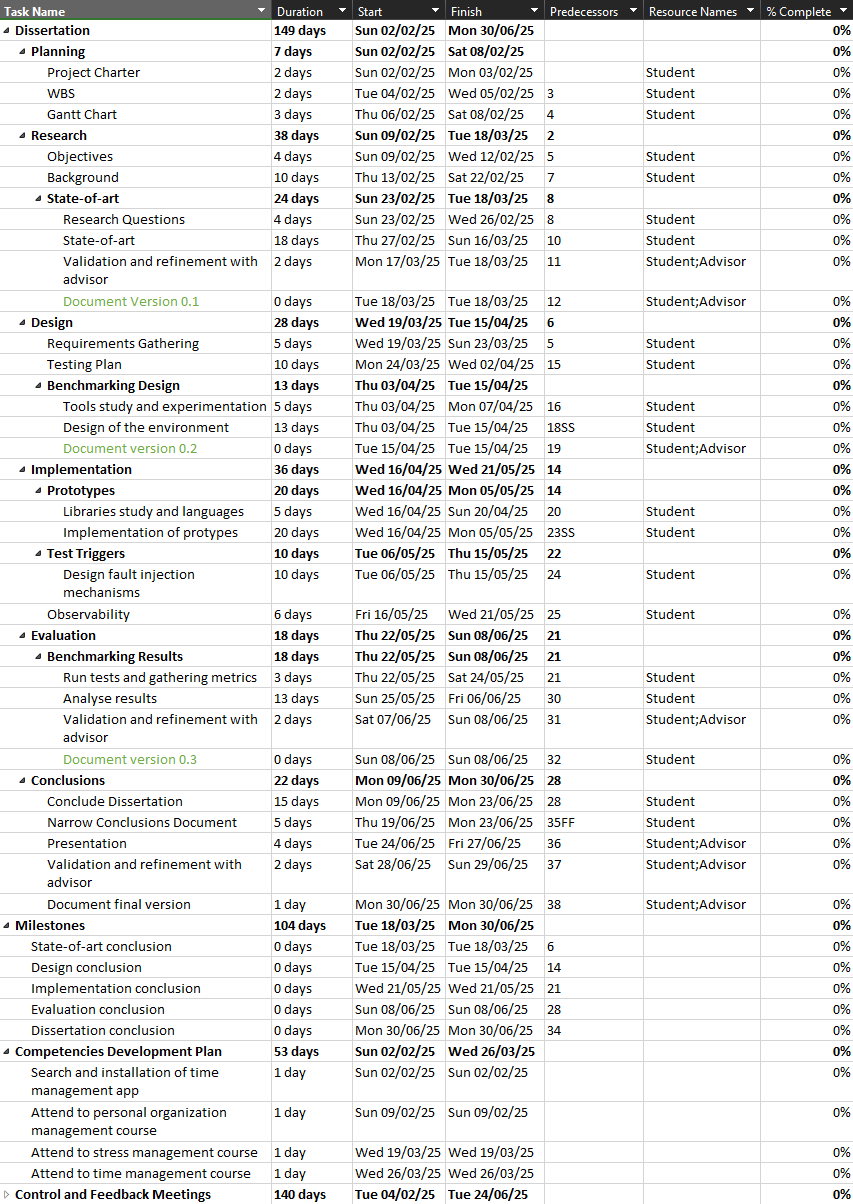
\includegraphics[width=\linewidth]{appendices/assets/gantt_complete.png}}
    \caption{Complete demonstration of the Gantt}
    \label{fig:gantt_complete}
\end{figure}

\section{Work Breakdown Structure Dictionary}

On the Table \ref{tab:wbs-dictionary} it is represented in a detailed way the description of the \gls{WBS}'s deliverables, such as the work loads. For each item there is a concise descriptions and a acceptance criteria.


\begin{longtable}{|p{3cm}|p{2.5cm}|p{8cm}|}
    \hline
    \textbf{Item Name}             & \textbf{Type of Item} & \textbf{Additional Description / Acceptance Criteria}                                                                                                                                                                                                                                                                                                     \\ \hline
    \endfirsthead
    \hline
    \textbf{Item Name}             & \textbf{Type of Item} & \textbf{Additional Description / Acceptance Criteria}                                                                                                                                                                                                                                                                                                     \\ \hline
    \endhead
    (1.1) Planning                 & Phase                 & This phase includes all initial project setup tasks.                                                                                                                                                                                                                                                                                                      \\ \hline
    (1.1.1) Project Charter        & Deliverable           & The project charter must be created following the project's scope and management guidelines. \newline \textbf{Acceptance Criteria:} The project charter must be approved by the advisor.                                                                                                                                                                  \\ \hline
    (1.1.2) \gls{WBS}              & Deliverable           & The \gls{WBS} should break down the project into manageable components. \newline \textbf{Acceptance Criteria:} The WBS should be validated by the advisor and include all project elements.                                                                                                                                                               \\ \hline
    (1.1.3) Gantt Chart            & Deliverable           & A detailed timeline outlining tasks, dependencies, competence development plan, milestones, and the dissertation deadline. \newline \textbf{Acceptance Criteria:} The Gantt chart must accurately reflect project phases and be reviewed by the advisor.                                                                                                  \\ \hline
    \hline 

    (1.2) Research                 & Phase                 & This phase focuses on gathering the required knowledge and literature to support the project.                                                                                                                                                                                                                                                             \\ \hline
    (1.2.1) Objectives             & Deliverable           & Clear objectives for the project, that must detail what are the excepted outcomes. \newline \textbf{Acceptance Criteria:} Objectives should align with the research goals and be validated by the advisor.                                                                                                                                                \\ \hline
    (1.2.2) Background             & Deliverable           & Research and summarize the background of fault tolerance in distributed systems and the distributed and concurrent programming languages.  \newline \textbf{Acceptance Criteria:} The background section should include sufficient theoretical content approved by the advisor, and must include a clear justification for the languages chosen.          \\ \hline
    (1.2.3) State-of-art           & Deliverable           & Review the current literature on fault tolerance in Elixir, Go, and Scala with Akka. Also, what are the latest techniques for benchmarking distributed and concurrent programming, and if there are already studies on this topic. \newline \textbf{Acceptance Criteria:} State-of-the-art review must highlight gaps and relevance to the project scope. \\ \hline
    \hline 

    (1.3) Design                   & Phase                 & This phase involves requirements gathering, testing plan, and benchmarking design.                                                                                                                                                                                                                                                                        \\ \hline
    (1.3.1) Requirements Gathering & Deliverable           & Collect requirements for the benchmarking and evaluation of fault tolerance aspects. \newline \textbf{Acceptance Criteria:} Requirements must be detailed, reviewed, and approved by the advisor.                                                                                                                                                         \\ \hline
    (1.3.2) Testing Plan           & Deliverable           & A plan for testing different fault tolerance strategies and mechanisms in Elixir, Go, and Scala with Akka. \newline \textbf{Acceptance Criteria:} Testing plan must include scenarios and validation methods, reviewed by the advisor.                                                                                                                    \\ \hline
    (1.3.3) Benchmarking Design    & Deliverable           & Define the design for benchmarking environments. \newline \textbf{Acceptance Criteria:} Benchmarking environments design must be validated by the advisor, and must adhere to the test plan created.                                                                                                                                                      \\ \hline
    \hline

    (1.4) Implementation           & Phase                 & This phase involves the development of benchmarking prototypes.                                                                                                                                                                                                                                                                                           \\ \hline
    (1.4.1) Prototypes             & Deliverable           & Develop prototypes in Elixir, Go, and Scala with Akka for fault tolerance testing. \newline \textbf{Acceptance Criteria:} Prototypes must meet the test plan previously created and must be supported on the benchmarking design planned.                                                                                                                 \\ \hline
    (1.4.2) Test Triggers          & Deliverable           & Create fault injection mechanisms for testing fault tolerance. \newline \textbf{Acceptance Criteria:} Fault injection methods must simulate real-world scenarios and be validated by tests.                                                                                                                                                               \\ \hline
    (1.4.3) Observability          & Deliverable           & Implement observability tools for monitoring system behavior during tests. \newline \textbf{Acceptance Criteria:} Observability setup must capture the metrics defined on the test validations methods.                                                                                                                                                   \\ \hline
    \hline 

    (1.5) Evaluation               & Phase                 & Evaluate the results of the benchmarking tests.                                                                                                                                                                                                                                                                                                           \\ \hline
    (1.5.1) Benchmarking Result    & Deliverable           & Analyze and document the outcomes of benchmarking fault tolerance aspects. \newline \textbf{Acceptance Criteria:} Results must be clear, reproducible, and reviewed by the advisor.                                                                                                                                                                       \\ \hline
    \hline 

    (1.6) Conclusions              & Phase                 & Finalize and present the results of the dissertation.                                                                                                                                                                                                                                                                                                     \\ \hline
    (1.6.1) Dissertation           & Deliverable           & Compile the dissertation document with findings and analyses. \newline \textbf{Acceptance Criteria:} Dissertation must meet academic formatting and content guidelines.                                                                                                                                                                                   \\ \hline
    (1.6.2) Conclusions            & Deliverable           & Write concise conclusions summarizing key findings from the research, with the goal of creating a guide for future developers consult. \newline \textbf{Acceptance Criteria:} Conclusions must be concise and detail what are the cons and pros of using each language for each specific case, so that develops can easily decide.                        \\ \hline
    (1.6.3) Presentation           & Deliverable           & Prepare and deliver the final presentation to the evaluation committee. \newline \textbf{Acceptance Criteria:} Presentation must be clear and precise.                                                                                                                                                                                                    \\ \hline
    \caption{\gls{WBS} dictionary}
    \label{tab:wbs-dictionary}
\end{longtable}
%\input{appendices/appendixB}
%\input{appendices/appendixC}

\end{appendices}
%----------------------------------------------------------------------------------------

\end{document}
